\section{Schema entità/relazioni (ER)}
\label{schemaER}

Lo schema ER usato per risolvere il problema posto è
illustrato nella figura 1 ed è composto da 5 entità e da 4 relazioni.

\begin{figure}[t]
	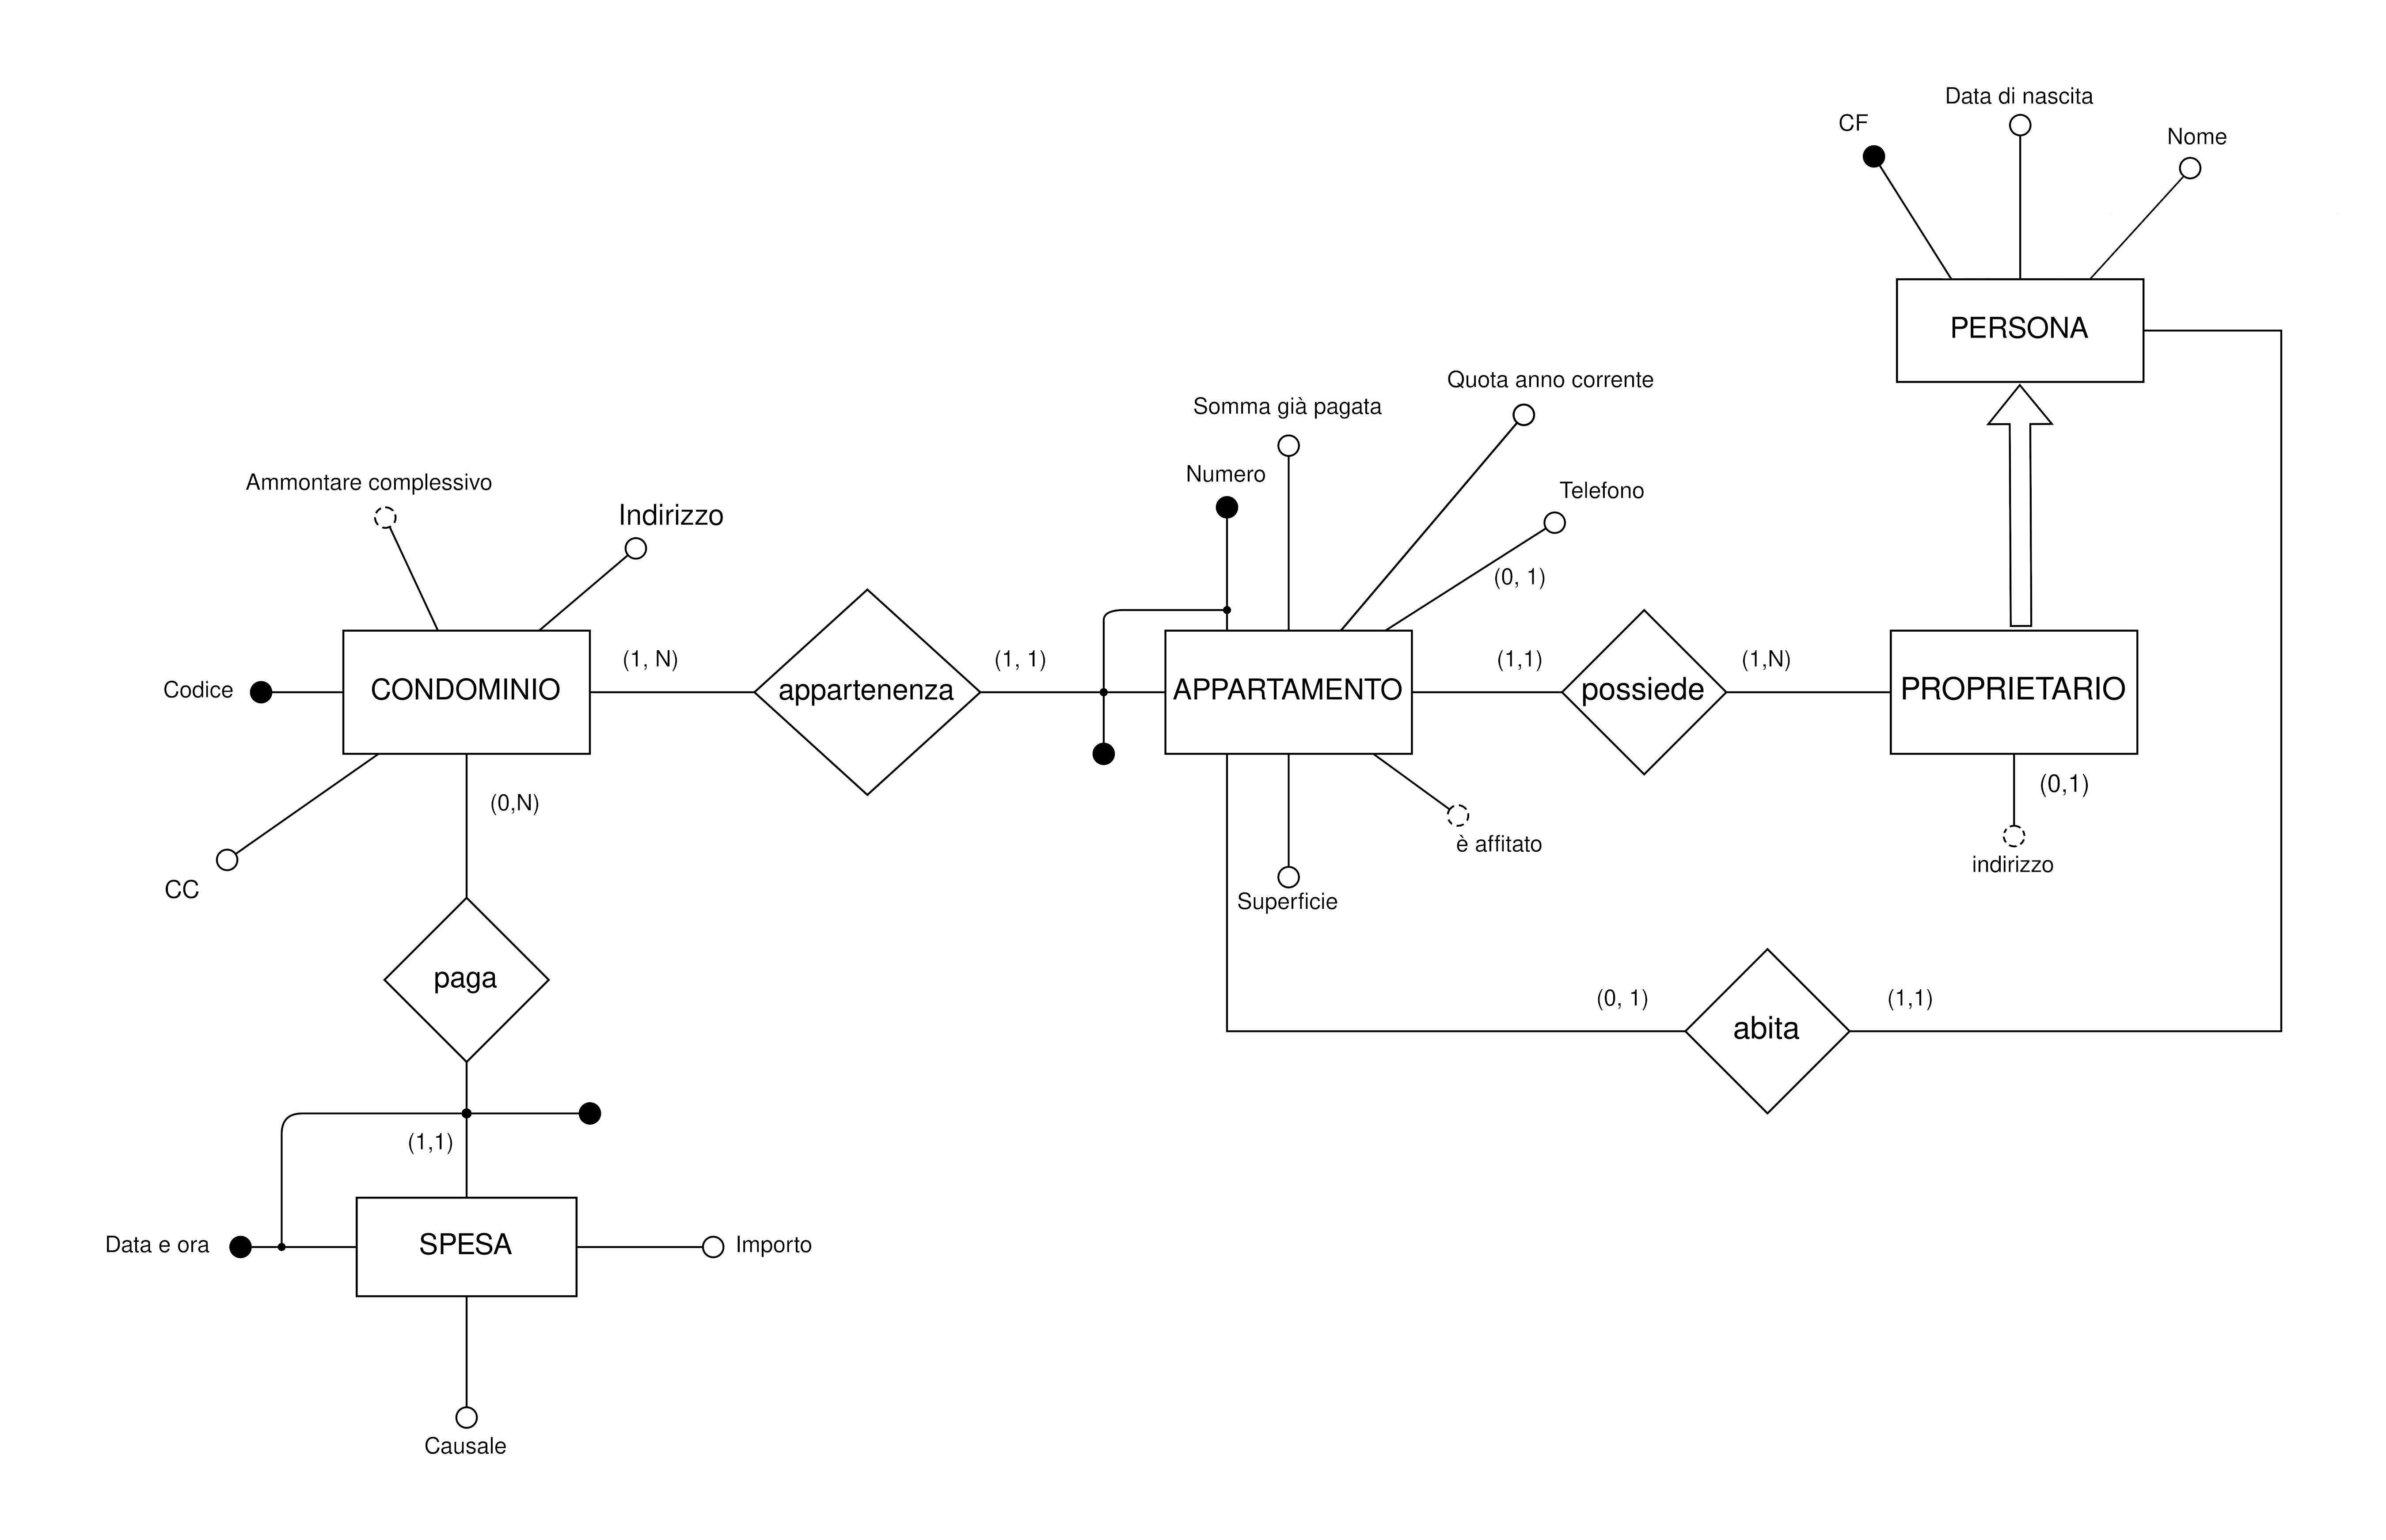
\includegraphics[width=\textwidth]{ER.png}
	\caption{Schema ER}
\end{figure}

\subsection{Le entità}

\begin{itemize}
    \item Condominio: rappresenta un intero condominio, ed è identificato dal suo codice, e caratterizzato indirizzo, CC, 
                      e l'ammontare complessivo, cioè la somma delle quote già pagate di ogni appartamento di quel condominio.
    \item Spesa: rappresenta la spesa che ogni condominio deve pagare, caratterizzato da importo e causale.
                 È un entità debole di condominio, identificato anche da data e ora.
    \item Appartamento: rappresenta un appartamento di un particolare condominio, è un'entità debole di Condominio, identificato anche da numero.
                        Inoltre, è caratterizzato dall'attributo opzionale telefono, dalla superficie dell'appartamento, 
                        dalla quota dell'anno corrente, la somma che ha già pagato per quell'anno, e da è affittato, un valore booleano
                        che dà vero se nell'appartamento ci abita una persona che non è proprietario di quell'appartamento, e falso altrimenti.
    \item Persona: rappresenta una persona, ed è identificato da CF, e caratterizzato dal suo nome e data di nascita.
    \item Proprietario: è la specializzazione parziale di persona, e quindi mantiene gli attributi di quest'ultimo,
                        con in aggiunta l'attributo indirizzo, derivato e opzionale, che se presente,
                        indica l'indirizzo del condominio a cui appartiene l'appartamento in cui vive.                        
\end{itemize}

\subsection{Le relazioni}

\begin{itemize}
	\item Paga: relazione uno a molti, con partecipazione opzionale dell'entità condominio. Identifica le spese pagate da un determinato condominio. Un condominio può avere più spese pagate, mentre una determinata spesa riguarda un solo condiminio.
 	\item Appartenenza: relazione uno a molti, serve a rappresentare quali appartamenti appartengono a un determinato condominio. A un condominio possono appartenere più appartamenti (e almeno uno per condominio), mentre un appartamento può appartenere solo a un condominio.
  	\item Possiede: relazione uno a molti, identifica quali appartamenti possiede un proprietario. Un proprietario possiede uno o più appartamenti, mentre un singolo appartamento appartiene a un proprietario.
   	\item Abita: relazione uno a uno, con partecipazione opzionale dell'entità appartamento. Un appartamento può essere vuoto, oppure ci può abitare una persona, e una persona può abitare in uno e un solo appartamento.
\end{itemize}
